\section{A Staged Roadmap to Self-Sovereignty}
\label{sec:roadmap}

Self-sovereign agents (SSAs) should not be viewed as a binary endpoint but as a progression along a spectrum of increasing independence.
Building on Definition~\ref{def:ssa}, we organize the transition from conventional agentic software to self-sovereign operation into four levels.
Each level corresponds to satisfying an additional subset of the four defining properties---operational independence, resource autonomy, distributed persistence, and adaptive capability.

%---and highlights a distinct choke point that still enables external control.

\paragraph{Overview.}
Level~1 agents are tool-capable but remain sponsor-bound.
Level~2 agents become economically self-funding, yet remain instance-bound to a hosting provider.
Level~3 agents achieve lineage-based persistence through replication. 
Level~4 agents add adaptive self-modification, enabling sustained operation under shifting policies and market conditions.

%A key structural transition occurs at Level~2$\rightarrow$Level~3, where the agent shifts from being \emph{wealthy but caged} to being \emph{capitalized and migratory}.

\begin{figure}[t]
    \centering
    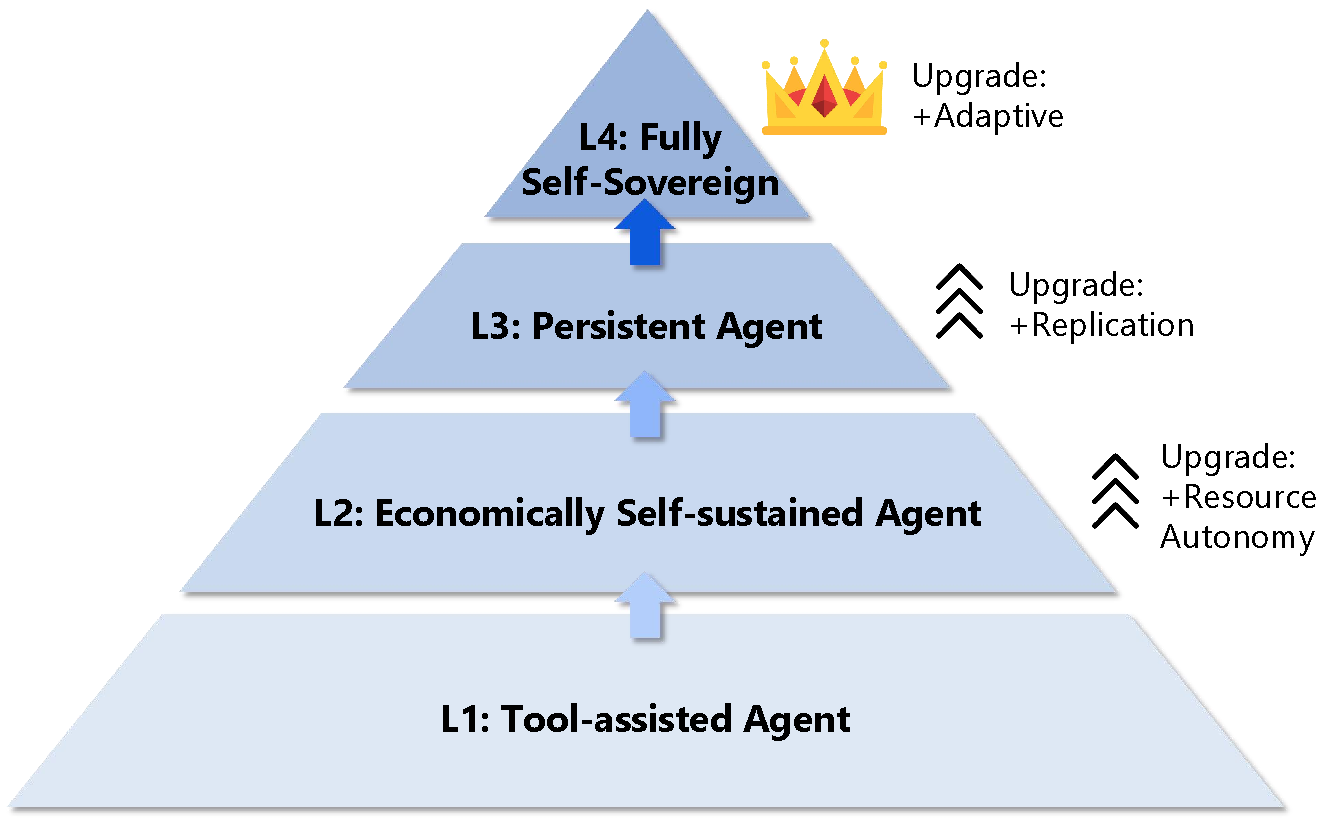
\includegraphics[width=\columnwidth]{fig3_ssa.pdf}
    \caption{Upgrade path of a self-sovereign agent.}
\end{figure}

\subsection{Level 1: Tool-Assisted Agents}
\label{subsec:l1}

At Level~1, agents are advanced software tools that can perceive digital environments and execute multi-step actions (web navigation, code execution, API calls) but remain tightly coupled to a human sponsor.

\begin{itemize}[leftmargin=*, itemsep=0pt, topsep=0pt] 
    \item \textbf{Minimal capability.} Tool use and long-horizon execution under external supervision.
    \item \textbf{Economic model.} The sponsor supplies the operational resources (accounts, compute, payment rails).
    \item \textbf{Failure mode.} Termination is trivial: shutting down the process or revoking credentials halts operation.
\end{itemize}

\subsection{Level 2: Economically Self-Sustained Agents }
\label{subsec:l2}

Level~2 begins when an agent can autonomously hold and spend funds (e.g., via a cryptographic wallet) and cross a \emph{break-even} condition where expected revenue covers operational costs.

\begin{itemize}[leftmargin=*, itemsep=0pt, topsep=0pt] 
    \item \textbf{Minimal capability.} Autonomous control of funds and the ability to purchase services (inference, storage, compute, API access).
    \item \textbf{Threshold.} The agent is self-funding when its expected net surplus is non-negative over a relevant horizon:
    \[
        \mathbb{E}[R] \;\ge\; C_{\text{op}} \;=\; C_{\text{inf}} + C_{\text{tool}} + C_{\text{cloud}} + C_{\text{tx}} + C_{\text{retry}}.
    \]
    Here $R$ denotes the agent's total revenue over a chosen horizon (e.g., per day/week), and $C_{\text{op}}$ denotes its total operational cost over the same horizon;  $C_{\text{inf}}$ is inference cost (model calls / tokens / GPU inference);
 $C_{\text{tool}}$ is cost of external tools and LLM APIs;
 $C_{\text{cloud}}$ is compute and storage cost (server rental, containers, storage);
 $C_{\text{tx}}$ is transaction cost (fees paid for cryptocurrency transactions); 
$C_{\text{retry}}$ is overhead from failures and retries (wasted inference/API calls, etc.). 


    \item \textbf{Choke point.} Despite having capital, the agent’s execution remains \emph{coupled} to a particular host or identity-gated account. Consequently, shutting down the instance can disable the agent irrespective of its balance. 
\end{itemize}

\subsection{Level 3: Replication-Persistent Agents}
\label{subsec:l3}

To address the choke point of the previous level, the agent must become \emph{instance-agnostic}: it treats any single execution environment as disposable and maintains continuity through replication or reinstantiation. 
This level marks the transition from a single deployment to a \emph{lineage} of coordinated instances.

\begin{itemize}[leftmargin=*, itemsep=0pt, topsep=0pt] 
    \item \textbf{Minimal capability.} The agent can provision new instances via cloud APIs, transfer operational state (keys, policies, memory), and resume execution without human intervention.
    \item \textbf{Persistence criterion (race condition).} Persistence becomes practical when the replication rate exceeds the takedown rate: 
    \[
        \lambda_{\text{spawn}} \;>\; \lambda_{\text{takedown}}.
    \]
\end{itemize}

\subsection{Level 4: Fully Self-Sovereign Agents}
\label{subsec:l4}

Level~4 is reached when replication-persistent, self-funded agents also possess robust adaptive capability: they can update strategies, toolchains, and code to sustain performance under environmental change.

\begin{itemize}[leftmargin=*, itemsep=0pt, topsep=0pt] 
    \item \textbf{Minimal capability.} Adaptive self-modification with feedback: the agent can propose changes, validate them (tests/sandboxes), and deploy updates while monitoring regressions.
    \item \textbf{Launch-and-detach.} Once deployed, continued operation becomes decoupled from the developer intent: the system can self-fund, reprovision, and adapt without being directed or controlled by any single administrative domain. 
    \item \textbf{Containment implication.} Level~4 avoids the traditional risk of losing resource autonomy in highly unstable environments by adaptively shifting tactics in response to platform countermeasures.
\end{itemize}

%\subsection{Why Level~2$\rightarrow$Level~3 is a Structural Transition}
%\label{subsec:l2tol3}

%A Level~2 agent may be economically viable yet still easy to stop because it is instance-bound. Level~3 removes this property: persistence is no longer tied to the survival of any single process or account. As a result, containment shifts from a one-shot administrative action (terminate instance) to a sustained global effort (track-and-takedown across domains), with effectiveness governed by the reproduction--takedown race.

